\documentclass[journal,12pt,twocolumn]{IEEEtran}
\usepackage{romannum}
\usepackage{float}
\usepackage{setspace}
\usepackage{gensymb}
\singlespacing
\usepackage[cmex10]{amsmath}
\usepackage{amsthm}
\usepackage{mathrsfs}
\usepackage{txfonts}
\usepackage{stfloats}
\usepackage{bm}
\usepackage{cite}
\usepackage{cases}
\usepackage{subfig}
\usepackage{longtable}
\usepackage{multirow}
\usepackage{enumitem}
\usepackage{mathtools}
\usepackage{steinmetz}
\usepackage{tikz}
\usepackage{circuitikz}
\usepackage{verbatim}
\usepackage{tfrupee}
\usepackage[breaklinks=true]{hyperref}
\usepackage{tkz-euclide}
\usetikzlibrary{calc,math}
\usepackage{listings}
    \usepackage{color}                                            %%
    \usepackage{array}                                            %%
    \usepackage{longtable}                                        %%
    \usepackage{calc}                                             %%
    \usepackage{multirow}                                         %%
    \usepackage{hhline}                                           %%
    \usepackage{ifthen}                                           %%
  %optionally (for landscape tables embedded in another document): %%
    \usepackage{lscape}     
\usepackage{multicol}
\usepackage{chngcntr}
\DeclareMathOperator*{\Res}{Res}
\renewcommand\thesection{\arabic{section}}
\renewcommand\thesubsection{\thesection.\arabic{subsection}}
\renewcommand\thesubsubsection{\thesubsection.\arabic{subsubsection}}

\renewcommand\thesectiondis{\arabic{section}}
\renewcommand\thesubsectiondis{\thesectiondis.\arabic{subsection}}
\renewcommand\thesubsubsectiondis{\thesubsectiondis.\arabic{subsubsection}}

% correct bad hyphenation here
\hyphenation{op-tical net-works semi-conduc-tor}
\def\inputGnumericTable{}                                 %%

\lstset{
frame=single, 
breaklines=true,
columns=fullflexible
}

\begin{document}


\newtheorem{theorem}{Theorem}[section]
\newtheorem{problem}{Problem}
\newtheorem{proposition}{Proposition}[section]
\newtheorem{lemma}{Lemma}[section]
\newtheorem{corollary}[theorem]{Corollary}
\newtheorem{example}{Example}[section]
\newtheorem{definition}[problem]{Definition}
\newcommand{\BEQA}{\begin{eqnarray}}
\newcommand{\EEQA}{\end{eqnarray}}
\newcommand{\define}{\stackrel{\triangle}{=}}

\bibliographystyle{IEEEtran}
\providecommand{\mbf}{\mathbf}
\providecommand{\pr}[1]{\ensuremath{\Pr\left(#1\right)}}
\providecommand{\qfunc}[1]{\ensuremath{Q\left(#1\right)}}
\providecommand{\sbrak}[1]{\ensuremath{{}\left[#1\right]}}
\providecommand{\lsbrak}[1]{\ensuremath{{}\left[#1\right.}}
\providecommand{\rsbrak}[1]{\ensuremath{{}\left.#1\right]}}
\providecommand{\brak}[1]{\ensuremath{\left(#1\right)}}
\providecommand{\lbrak}[1]{\ensuremath{\left(#1\right.}}
\providecommand{\rbrak}[1]{\ensuremath{\left.#1\right)}}
\providecommand{\cbrak}[1]{\ensuremath{\left\{#1\right\}}}
\providecommand{\lcbrak}[1]{\ensuremath{\left\{#1\right.}}
\providecommand{\rcbrak}[1]{\ensuremath{\left.#1\right\}}}
\theoremstyle{remark}
\newtheorem{rem}{Remark}
\newcommand{\sgn}{\mathop{\mathrm{sgn}}}
\providecommand{\abs}[1]{\left\vert#1\right\vert}
\providecommand{\res}[1]{\Res\displaylimits_{#1}} 
\providecommand{\norm}[1]{\left\lVert#1\right\rVert}
\providecommand{\mtx}[1]{\mathbf{#1}}
\providecommand{\mean}[1]{E\left[ #1 \right]}
\providecommand{\fourier}{\overset{\mathcal{F}}{ \rightleftharpoons}}
\providecommand{\system}{\overset{\mathcal{H}}{ \longleftrightarrow}}
\newcommand{\solution}{\noindent \textbf{Solution: }}
\newcommand{\cosec}{\,\text{cosec}\,}
\providecommand{\dec}[2]{\ensuremath{\overset{#1}{\underset{#2}{\gtrless}}}}
\newcommand{\myvec}[1]{\ensuremath{\begin{pmatrix}#1\end{pmatrix}}}
\newcommand{\mydet}[1]{\ensuremath{\begin{vmatrix}#1\end{vmatrix}}}
\numberwithin{equation}{subsection}
\makeatletter
\@addtoreset{figure}{problem}
\makeatother

\let\StandardTheFigure\thefigure
\let\vec\mathbf
\renewcommand{\thefigure}{\theproblem}



\def\putbox#1#2#3{\makebox[0in][l]{\makebox[#1][l]{}\raisebox{\baselineskip}[0in][0in]{\raisebox{#2}[0in][0in]{#3}}}}
     \def\rightbox#1{\makebox[0in][r]{#1}}
     \def\centbox#1{\makebox[0in]{#1}}
     \def\topbox#1{\raisebox{-\baselineskip}[0in][0in]{#1}}
     \def\midbox#1{\raisebox{-0.5\baselineskip}[0in][0in]{#1}}

\vspace{3cm}


\title{Assignment 1}
\author{Jaswanth Chowdary Madala}





% make the title area
\maketitle

\newpage

%\tableofcontents

\bigskip

\renewcommand{\thefigure}{\theenumi}
\renewcommand{\thetable}{\theenumi}



\begin{enumerate}
\item A die is thrown, find the probability of following events:
\begin{enumerate}
\item A prime number will appear
\item A number greater than or equal to 3 will appear
\item A number less than or equal to one will appear
\item A number more than 6 will appear
\item A number less than 6 will appear
\end{enumerate}
\textbf{Solution:} The given information is summarized in the following table \ref{tab:1}
\begin{table}[h]
\centering
%%%%%%%%%%%%%%%%%%%%%%%%%%%%%%%%%%%%%%%%%%%%%%%%%%%%%%%%%%%%%%%%%%%%%%
%%                                                                  %%
%%  This is a LaTeX2e table fragment exported from Gnumeric.        %%
%%                                                                  %%
%%%%%%%%%%%%%%%%%%%%%%%%%%%%%%%%%%%%%%%%%%%%%%%%%%%%%%%%%%%%%%%%%%%%%%

\begin{center}
\begin{tabular}{|c|c|c|}
\hline
\textbf{RV}& \textbf{Values} & \textbf{Description} \\ \hline
$X$		   & 	$\{0,1\}$	&  1st draw - 0: black card, 1: red card\\ \hline
$Y$ 		   & 	$\{0,1\}$	&  2nd draw - 0: black card, 1: red card\\ \hline
$X,Y$ 		   & 	$\{00\}$	&	2 cards drawn are black\\ \hline
\end{tabular}
\end{center}

\caption{Random variable X}
\label{tab:1}
\end{table}
\begin{figure}[ht]
\centering
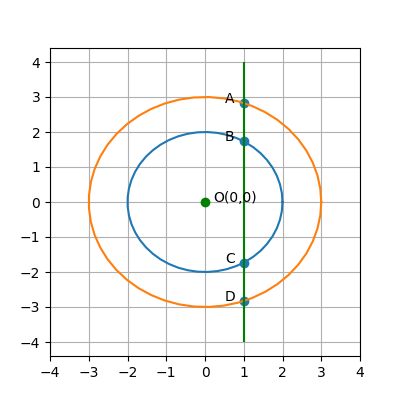
\includegraphics[width = \columnwidth]{"figs/fig.png"}
\caption{Graph}
\label{fig:1}
\end{figure}

The CDF of the random variable $X$ is given by,
\begin{align}
F_{X}\brak{n} = 
\begin{cases}
0 & n < 1 \\
\frac{[n]}{6} & 1 \le n \leq 6 \\
1 & \text{otherwise}
\end{cases}
\end{align}
where [.] denotes Greatest Integer function. The graph of the CDF function is shown in the figure 
%\begin{align}
%F_{X}\brak{n} = 
%\begin{cases}
%0 & n < 1 \\
%\frac{1}{6} & 1 \le n < 2 \\
%\frac{1}{3} & 2 \le n < 3 \\
%\frac{1}{2} & 3 \le n < 4 \\
%\frac{2}{3} & 4 \le n < 5 \\
%\frac{5}{6} & 5 \le n < 6 \\
%1 & \text{otherwise}
%\end{cases}
%\end{align}
\begin{enumerate}
\item The set of possible prime numbers in a die roll contains 2,3,5
\begin{align} 
\pr{X \in \{2,3,5\}} &= \pr{X = 2} + \pr{X = 3} + \pr{X = 5}\\
&= \frac{1}{2}
\end{align}
\item The probability that a number greater than or equal to 3 will appear is given by
\begin{align}
\pr{X \geq 3} &= 1 - \pr{X \leq 2}\\
&= 1 - F_{X}\brak{2}\\
&= \frac{2}{3}
\end{align}
\item The probability that a number less than or equal to 1 will appear is given by
\begin{align}
\pr{X \leq 1} &= F_{X}\brak{1}\\
&= \frac{1}{6}
\end{align}
\item The probability that a number greater than 6 will appear is given by
\begin{align}
\pr{X > 6} &= 1 - \pr{X \leq 6}\\
&= 1 - F_{X}\brak{6}\\
&= 0
\end{align}
\item The probability that a number less than 6 will appear is given by
\begin{align}
\pr{X < 6} &= \pr{X \leq 5}\\
&= F_{X}\brak{5}\\
&= \frac{5}{6}
\end{align}
\end{enumerate}
\end{enumerate}
\end{document}



